\documentclass{article}
\usepackage[margin=1in]{geometry}
\usepackage{roboto}
\usepackage{xcolor}
\usepackage{colortbl}
\usepackage{graphicx}

\definecolor{lightgrey}{HTML}{ECECEC}

\begin{document}

\begin{center}
    {\fontsize{28}{36}\selectfont\bfseries MVTR Adventure Bike Rally Difficulty}
\end{center}

\vspace{1em}

\noindent
\begin{minipage}{0.45\linewidth}
    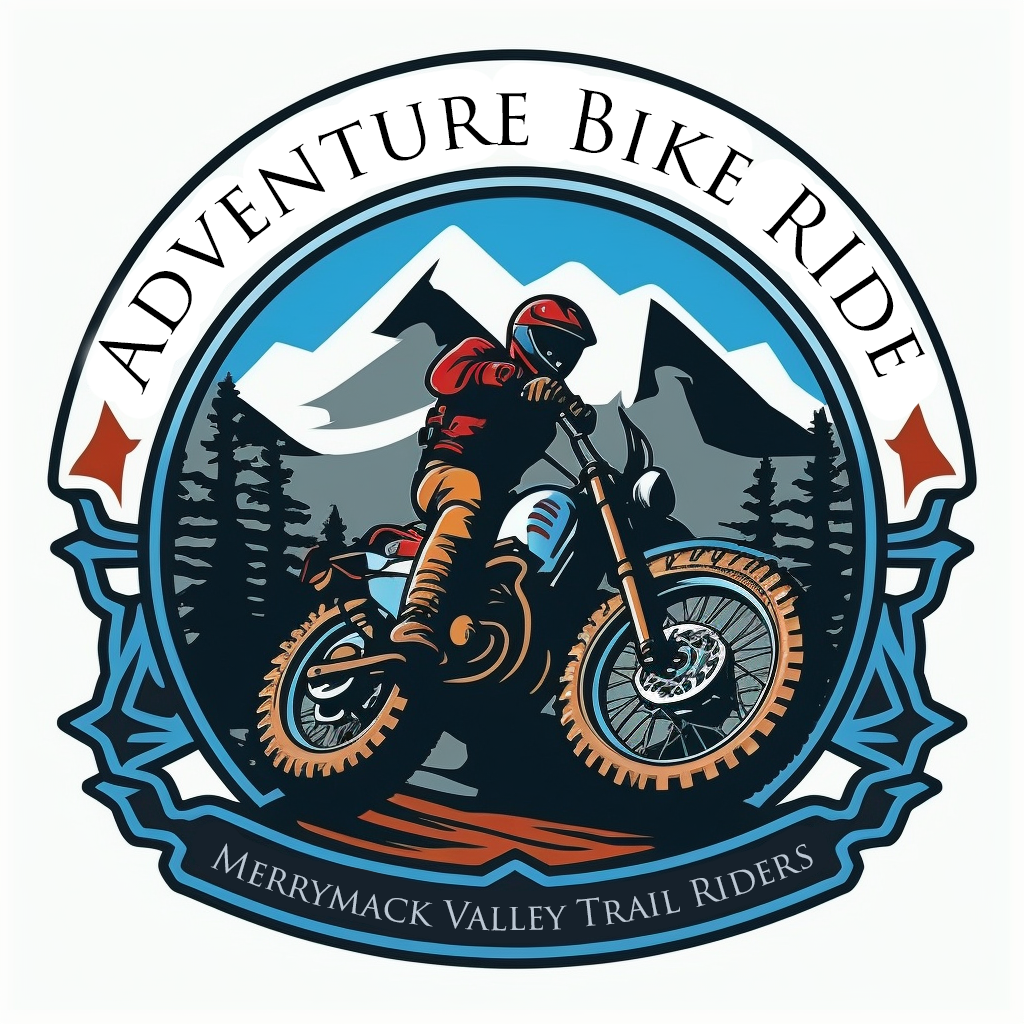
\includegraphics[width=\linewidth]{temp_logo.png}
\end{minipage}%
\begin{minipage}{0.5\linewidth}
    \setlength{\fboxsep}{10pt}
    \setlength{\fboxrule}{2pt}
    \fcolorbox{black}{white}{%
        \begin{minipage}[t]{\linewidth}
            \textbf{Important Information}

            \vspace{0.5em}
            \textbf{Tires} \\
            50:50 tires should be considered a minimum for rides. All of our routes have extensive off-pavement sections and riding street-oriented tires just puts the rest of the group at risk of unfortunate delays. \textbf{Anything above level II should not be attempted without proper knobbies}.

            \vspace{1.5em}

            \textbf{Physical Fitness} \\
            \noindent Physical Fitness plays a significant role in adventure riding. Rides take up to 8 hours and can have sustained levels of difficulty. If you find yourself on a route that challenges your skills, we are never far from any exit route. Weather can also play a significant role in the difficulty of a route.
        \end{minipage}%
    }
\end{minipage}%

\hfill%

\begin{minipage}[t]{0.9\linewidth}
    \textbf{Difficulty Levels}

    Consider that the difficulty of a route is not just about the terrain, but also the weather, the group, and your own skill level. The difficulty level is a guide to help you choose an adventure that is appropriate for your skills and abilities. If you are unsure, ask a ride leader for advice.
    \vspace{0.2em}
    The routes are laid out with an \textit{choose your own adventure} style in mind. The guided groups will roughly follow one of the levels (you always have the option of skipping Hero sections, even in the guided groups).
    \vspace{0.5em}

    \begin{center}
        \begin{tabular}{|c|p{12cm}|}
            \hline
            \textbf{Level} & \textbf{Description}                                                                                                                                                                                                                                                                                                                                                                            \\
            \hline
            I              & Rough paved roads with broken bits, potholes, and mud. Well maintained gravel roads.                                                                                                                                                                                                                                                                                                            \\
            \hline
            II             & Rough resource roads. Smooth double track. Small and infrequent trail obstacles. Patches of soft gravel, shallow sand, or small surface mud. All hills are gentle. \textbf{OFF-ROAD EXPERIENCE RECOMMENDED}                                                                                                                                                                                     \\
            \hline
            III            & Doubletrack with routine modest features such as roots, rocks, and soft patches. Some steep hills, but short in duration. \textbf{OFF-ROAD EXPERIENCE STRONGLY RECOMMENDED}                                                                                                                                                                                                                     \\
            \hline
            IV             & All the above \& Doubletrack with routine features such as roots, ledges, rocks, and soft patches. Singletrack with infrequent obstacles. Elevation changes and mud are common. \textbf{OFF-ROAD EXPERIENCE REQUIRED}                                                                                                                                                                           \\
            \hline
            V              & All the above \& Single and double track with frequent and potentially sizable features such as roots, ledges, rocks, and soft patches. Some obstacles require commitment and don't have easy by-passes. Steep hills can be sustained and may have unforgiving transitions. Corners may be tight and unforgiving. Mud holes and water crossings. \textbf{ADVANCED OFF-ROAD EXPERIENCE REQUIRED} \\
            \hline
            \rowcolor{lightgrey}
            VI             & All the above \& Challenging for dirt bikers, so yeah, it’s really tough for anything bigger. Make sure you can ride a few Level V routes before trying a Level VI.   \textbf{YOU KNOW WHAT YOU'RE DOING AND YOU'RE ASKING FOR IT}                                                                                                                                                              \\
            \hline
            % \rowcolor{lightgrey}
            % VII              & Extremely challenging routes, even for the very best riders on smaller adventure bikes. Unavoidable large obstacles requiring significant commitment and potentially some nasty exposure. Train hard to possibly do one someday so you can tick that box, and never have to do another again! \\
            % \hline
        \end{tabular}
    \end{center}
\end{minipage}

\end{document}
